\documentclass{amsart}

\usepackage[brazilian]{babel}
\usepackage[utf8]{inputenc}
\usepackage{graphicx}
\usepackage{mathtools}
\usepackage{amsthm}
\usepackage{amsfonts}
\usepackage{hyperref}
\usepackage[singlelinecheck=false]{caption}
\usepackage{enumitem}
\usepackage[justification=centering]{caption}
\usepackage{indentfirst}
\usepackage{listings}

\makeatletter
\def\subsection{\@startsection{subsection}{3}%
  \z@{.5\linespacing\@plus.7\linespacing}{.1\linespacing}%
  {\normalfont\itshape}}
\makeatother

\DeclareMathOperator*{\argmin}{arg\,min}
\DeclareMathOperator*{\argmax}{arg\,max}

\newcommand\defeq{\mathrel{\overset{\makebox[0pt]{\mbox{\normalfont\tiny\sffamily def}}}{=}}}

\captionsetup[table]{labelsep=space}

\theoremstyle{plain}

\newtheorem*{definition}{Definição}
\newtheorem{theorem}{Theorem}
\newtheorem{proposition}{Proposition}
\newtheorem{exercise}{Exercise}

\newcommand{\set}[1]{\mathcal{#1}}
\newcommand{\pr}{\mathbb{P}}
\renewcommand{\implies}{\Rightarrow}

\lstset{frameround=fttt,
	language=C,
	numbers=left,
	breaklines=true,
	keywordstyle=\bfseries,
	basicstyle=\ttfamily,
	numberstyle=\color{black}
}

\lstMakeShortInline[columns=fixed]|

\setlength{\parskip}{1em}

\title[]{EP1 -- MAC0438 -- Programação Concorrente}
\author[]{Renato Lui Geh\\NUSP\@: 8536030}

\begin{document}

\begin{abstract}
  Soluções dos exercícios bônus do Exercício Programa 1 de MAC0438 Programação Concorrente.
  \vspace*{-2.5em}
\end{abstract}

\maketitle

\section{Diagramas}

Os diagramas serão apresentados como um grafo parcialmente direcionado. Cada aresta direcionada
representa a sequência de passos do processo local. Uma aresta não-direcionada é a criação de um
novo processo cujo pai é um subgrafo conectado à aresta. Um nó com formato de caixa é uma indicação
de um novo processo. Um processo acaba se este passa pelo nó |kill|. Para clarificar como
o grafo representa paternidade de processos, considere a definição abaixo:

\begin{definition}
  Um processo é um grafo direcional $H=(V_H,E_H)$. Um processo $H$ tem pai $G=(V_G,E_G)$ sse existe
  um nó $i\in V_H$ que tem formato de caixa e possue uma aresta não-direcionada $(i,j)$, onde
  $j\in V_G$. Diz-se então que $G$ é pai de $H$ e $H$ é filho de $G$. O grafo $H$ será chamado de
  subgrafo de processo.
\end{definition}

Vamos chamar esse diagrama como Grafo de Processos (GP). Um grafo direcional que possue um caminho
$(i,j)$ que passa somente por arestas direcionais é um processo. Todo subgrafo que possue tal
caminho é um processo do GP\@. Todas as folhas de um GP devem ser nós |kill|.

Por causa do tamanho dos grafos de processos, a explicação da análise estará separada dos grafos
de processos. A Seção~\ref{solutions} explica a análise, enquanto que a Seção~\ref{graphs} mostra
os grafos de processos.

\section{Soluções}~\label{solutions}

\subsection{Programa 1}

Neste programa são criados quatro processos filhos e um processo pai. O Grafo de Processos está
ilustrado na Figura~\ref{p1}.

Assim que é criado o primeiro processo filho, o processo pai entra na condição de sair do laço
|for|. No primeiro processo filho, este age como se fosse o processo pai, criando um novo processo
que é filho do primeiro processo filho recursivamente. Como o quarto processo filho tem |i=4|, ele
logo é eliminado do |for|, e portanto não cria processos filhos.

\subsection{Programa 2}

São criados quatro processos filhos e um processo pai. Considere a Figura~\ref{p2}.

É possível ver que, assim que criam-se todos os processos com |fork| nas quatro
iterações, o processo pai termina sua execução. Os processos filhos tem sua paternidade
automaticamente movida para o processo |init| pelo sistema operacional, o que guarante
que os processos continuem rodando. Assim que cada um acabar sua execução, a memória de cada
processo é liberada. Todos os processos filhos são criados pelo processo pai original.

\subsection{Programa 3}

São criados sete processos filhos e um processo pai desde que todos os processos consigam ser
criados. Como o Grafo de Processos ficaria muito grande, considere a árvore de recursão na
Figura~\ref{rec_tree}.

\begin{figure}[h]
  \centering{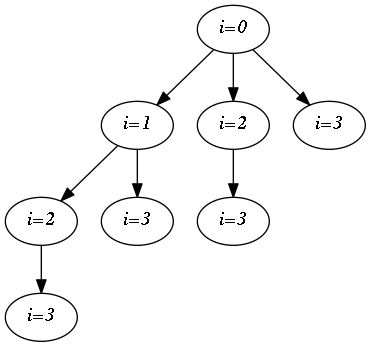
\includegraphics[scale=0.4]{graphs/p3.png}
  \caption{Árvore de recursão do Programa 3. Cada nó representa um processo. Uma aresta indica
  paternidade entre nós. A soma de todos os nós é a quantidade total de processos.}\label{rec_tree}
  }
\end{figure}

A criação dos processos é recursiva. Como o |for| acaba apenas se |i>=3| ou se o processo não
conseguiu ser criado, então cada processo cria uma quantidade de filhos $\mid i-3\mid$. A soma de
todos os nós é a quantidade de processos do programa. O número de filhos de um nó é o número de
processos filhos daquele processo. Como |i=0..3| no |for|, então $Ch(j)\leq 3$, onde $Ch(j)$ é o
conjunto de nós filhos do nó $j$. Um nó $i$ é filho de um nó $j$ se existe uma aresta direcionada
$j\rightarrow i$. O valor de um nó é o valor do contador |i| local do processo.

\section{Grafos de Processos}~\label{graphs}

\begin{figure}[h]
  \centering{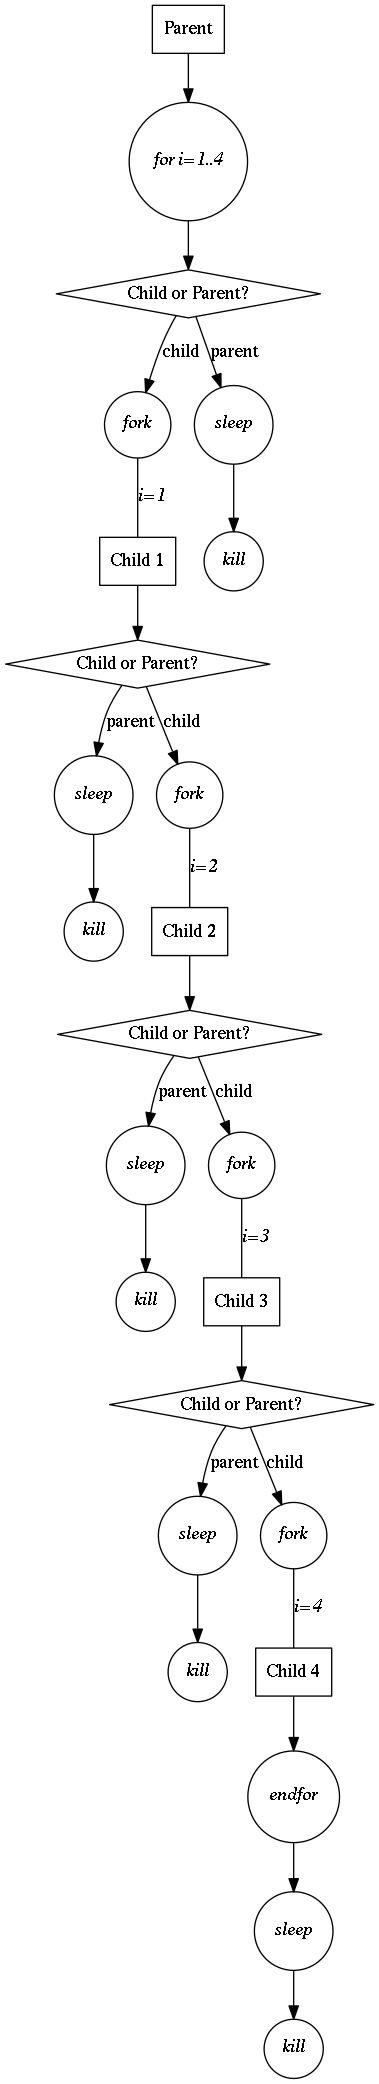
\includegraphics[scale=0.3]{graphs/p1.png}
  \caption{É possível ver que o grafo de processos é recursivo neste programa. Cada criação de
  processo gera um novo subgrafo de processo, que por sua vez cria um novo subgrafo de processo.}\label{p1}
  }
\end{figure}

\begin{figure}[h]
  \centering{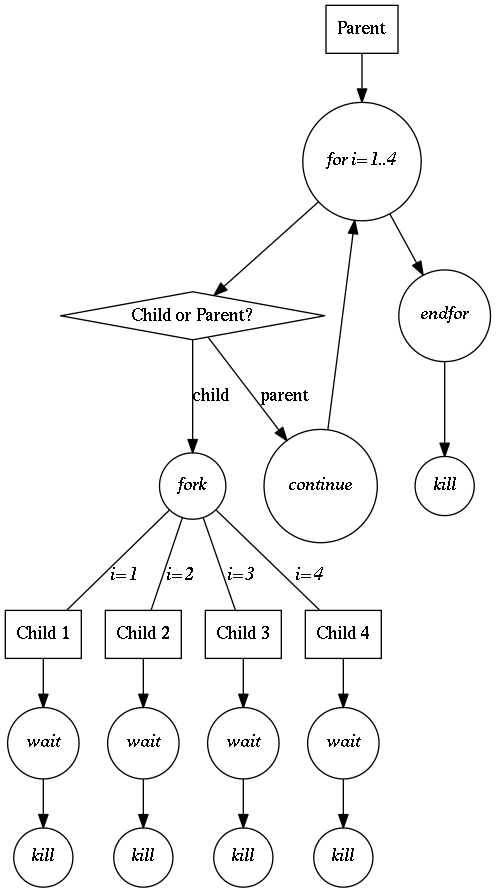
\includegraphics[scale=0.4]{graphs/p2.png}
  \caption{Neste GP, a criação de processos é iterativa. O processo pai percorre o laço criando
  processos filhos. Os filhos, por sua vez, não iteram pelo laço, já que estes caem na condição de
  serem filhos, quebrando o laço.}\label{p2}
  }
\end{figure}


\end{document}
